\section{Sentiment Analysis}
The cornerstone for this thesis is sentiment analysis and this topic requires the definition of a lot of terms and concepts that are important to the research at hand.
Sentiment Analysis in theory sounds rather simple, process text and pull out the meaning based on the content of what was processed, but there are many intricacies that need to be addressed to fully understand the entire process [\cite{liu2012sentiment}].

\subsection{Definition}
Sentiment Analysis refers to the use of natural language processing and text analysis to systematically identify, extract, quantify, and study affective states and subjective information [\cite{liu2012sentiment}].
Sentiment Analysis has increased in popularity in recent years and is popular to use to review large sets of review / survey data to abstract major topics of conversation and controversy online.
It can be an effective tool in summarizing a population's opinions and feelings towards certain issues and drawing conclusions from them.
A basic task of sentiment analysis that can be leveraged into more complex tasks is determining the polarity of a sample of text data and classify it as positive, negative, or neutral [\cite{wilson2005recognizing}].
The process behind sentiment analysis is important and can be complicated depending on how much information an analysis is trying to pull and how large of a dataset is involved, and before the process is addressed, there are certain principles and topics involved that need to be covered first.

\subsection{Natural Language Processing}
Natural Language Processing (NLP) is an important concept that is used heavily in sentiment analysis.
NLP is primarily concerned with the interactions between human beings and computers and specifically how they process and discern the meaning of human language [\cite{liddy2001natural}].
Natural Language Data is abundant in our world today in the Age of the Internet and the vastness of it makes NLP extremely important to implement effectively to aid in understanding this large dataset.
NLP takes on the difficult task of processing large text data and attempting to quantify the text data in different ways.

\subsubsection{Natural Language Toolkit}
NLP is the concept and the implementation in this project is the Natural Language Toolkit (NLTK), which is a Python library that offers NLP methods to process text and extract meaningful trends and patterns from the text of interest.
The NLTK is implemented using Python, which is a simple, yet powerful language with excellent functionality for processing linguistic data \cite{bird2004nltk}.
Much of the meaning is derived using the NLTK but much of the processing is conducted in purely Python using lists of words to process meaning and sentiment.
The task of processing text data comes with a few obstacles that can either obstruct meaning or complicate the processing by changing the meaning of words or phrases based on the context in which they reside.

\subsection{Complications with Text Data}
Text Data can be especially difficult to deal with and cause a lot of unforeseen issues when it is being processed.
The inherent subjectivity of human language and speech is one of the largest obstacles that must be addressed when dealing with any text-based data.
Much of the communication between human beings is subjective and it is up to the interpretation of the speaker and listener what the message is and they can have conflicting ideas on the meaning of some terms [\cite{aggarwal2012mining}].
This potential for miscommunication is mirrored in NLP in that the determined meaning or value of some textual data could not be representative of the source it came from, and there is not an objective reference to the weight of words to confirm the correctness of any one interpretation of the textual data.

Another important factor to consider when processing text data is sarcasm, which is extremely difficult to detect.
Americans especially are known for their use of sarcasm and it can be sometimes impossible to parse such meaning out of text since the intonation is what indicates the sarcasm which is lost in purely text-based data.
There are some subtle cues that can indicate sarcasm in text but it can really only consistently be caught if it is tagged as such [\cite{riloff2013sarcasm}].

A third and final complication that often arises is considering the context in which the text resides [\cite{aggarwal2012mining}].
Context is everything when examining how people speak and trying to accurately access the thoughts and opinions of the speaker so it is important to take this context into consideration when developing a sentiment analysis since it will affect any results that are achieved.
Context here meaning the modifying words surrounding the word to be examined next in the analysis.
Each word in a sample of text data can have any number of modifiers that can manipulate its meaning and fundamentally change what message it is conveying by adding certain words before or after the word.
These modifiers can take on the form of intensifiers, such as very, that amplify the meaning of a word, 

\subsection{Lexicon}
There are several ways to conduct sentiment analysis, some of which do not require a lexicon but this research used a lexicon-based approach.
An important tool that is necessary in conducting this analysis is a comprehensive lexicon.
A lexicon is a database of words and accompanying features associated with each word [\cite{taboada2011lexicon}].
These features associated with each word vary widely in what they say about the word, from part of speech to length to polarity score.
The lexicon used in this research consists of a word and an associated sentiment score that is on the scale from -1.0 (negative) to 1.0 (positive), indicating how positive or negative the word is.
These sentiment scores were compiled from several different lexicons and the results were compiled by surveying thousands of individuals and having them score a certain subset of words and combine those ratings into an average score for each word [\cite{somasundaran2010lexicon}].

\subsection{Alternative Sentiment Analysis Approaches}
There are other ways of conducting sentiment analysis without the use of a lexicon that can also be useful for conducting the analysis.
The main alternative method is a comparative approach that compares each block of text data to one another and instead of giving them an objective score, ranks them according to a subset of rules that determine their ranking relative to the other samples of text [\cite{wilson2005contextual}].
This approach puts much more focus on the context of what is being said and uses context to determine the polarity of language.
This is the main approach used by many political science researchers, since it is far easier to compare politician's values relative to one another than use an objective dictionary to determine their stance on an issue. [\cite{laver2003extracting}]

\subsection{Process}
The process behind sentiment analysis, especially when it is lexicon-based, is rather simple to understand but there are a lot of hidden factors that must be considered.
The most important and most influential part of this entire process is the lexicon, which was covered in the previous section.
The lexicon is used as the basis for all the sentiment scores that are assigned in the analysis, thus its integrity and accuracy is central to the success of the analysis.
The analysis is started by feeding in the text data to the program. 
In this case, that text data was the Presidential State of the Union Addresses.
This text data is split into an array, each index corresponding to an individual word.
At this point, the text data is cleaned up, using assorted algorithms to handle punctuation and capitalization and other linguistic features that could complicate the sentiment score assignment.
Once the data is cleaned, it is time to start the bulk of the sentiment score operation.
Using nested for-loops, each individual word is compared to a list of "common" words to avoid wasting time and processing power on "the" and other non-notable words, and then each non-common word is compared to the lexicon the score for that individual score is recorded in an overall score variable.
As each word is processed, this score variable is either incremented or decremented based on the value associated with said word in the lexicon, and also an overall counter variable is incremented each time, counting each individual word.
After all the words have been processed, the total score that has been tabulated is then divided by the counter and that resulting number is the sentiment score for that selection of text.
There are a couple of odds and ends that were glossed over that will be covered in the next sections since they were added after the initial algorithm was constructed that slightly influence it's behavior when encountering certain specialty words, and also classifying different topics within the body of text.

\begin{singlespace}
\begin{algorithm}[H]
\DontPrintSemicolon
\KwIn{All State of the Union Addresses}
\KwOut{The sentiment score for each Presidential Address for each category.}
\BlankLine
open all .txt files and store them in lists of special category trigger words\;
\For{each address in the State of the Union Addresses}
	{format address\;
	split address in to sentences\;
	\For{each sentence in the address}
		{add sentence to 'overall' category\;
		\If{sentence contains category trigger word}
		{add sentence to category}
	\For{each category}
		{append list of sentences for that category to an overall list}
	\For{each topic in the overall list}
		{\For{each word in the topic}
			{create word count for each word and store it in a dictionary\;
			\If{previous word negator}
				{increment negator counter for that word by one}
			\If{previous word intensifier}
				{increment intensifier counter for that word by one}
			}
		\For{each word in the dictionary}
		{\If{word is in lexicon}
		{\If{length of negators[word] != 0}
		{Subtract length from total count for that word}
		}
		\If{length of intensifiers[word] != 0}
		{Raise length number of scores to the power of 2}
		Calculate the Sentiment Score by multiplying the number of occurences of the term by the score in the lexicon.
		}
		}
	}
	}
	
\caption{Sentiment Analysis Algorithm}
\label{alg:one}
\end{algorithm}
\end{singlespace}

\subsubsection{Topic Classifier Sets}
An important part of the latter half of the preprocessing work for this research was the topic classifier sets.
At first, the sentiment score was calculated for each presidential address with an overall score from -1 to 1, indicating their tone when delivering that address.
After these were calculated, they were analyzed to look for trends in each president's tone to see if there were any interesting observations to be seen.
As an additional breakdown to see if there was any more context-specific information that could help determine a president's political party, topic categories were added to diversify the scores of the president's even more.

Four Presidential Addresses were chosen (Washington, Lincoln, Kennedy, Obama) and manually read through to discover what words were being used when talking about certain topics within the United States. The topics that were chosen were: crime, economy, education, energy, environment, family, foreign, government, job, religion, terrorism, and war. Text files were created using the trigger words for each major topic, the trigger words being pulled from the four addresses mentioned above and throughout various other addresses as they were skimmed through, that would add the entire sentence to an array named for what topic it was going to collect information on. This processing was conducted on every address and the sentiment score for each topic was found for each president, which resulted in a vector for each address that had their overall sentiment score and the sentiment score for each topic covered in the address. These scores for each address were then averaged together to create an overall vector for each president that could be used for classification and learning to learn their political party and predict others.

\section{Information Visualization}
An important part of this research is also concerned with how best to display the resulting information in an effective and easy-to-understand manner.
There is an entire field dedicated to how to best display technical information and data and how to convey it to large groups of people with little technical background [\cite{fekete2008value}].
This is important with data such as the sentiment score being processed here, as the long numbered sentiment scores are intimidating and without any context, data is meaningless.
The context here is contained within the graph used to display the sentiment score data and interactive features were implemented to help users engage with the data in a more meaningful fashion.
The data in this research is quantitative and since the Presidential Addresses are given in chronological order, time was used on the x-axis and the data lended itself nicely to a Line Plot.
This line plot will be discussed more in-depth in the following section.

\subsection{Line Plot}
\begin{figure}
  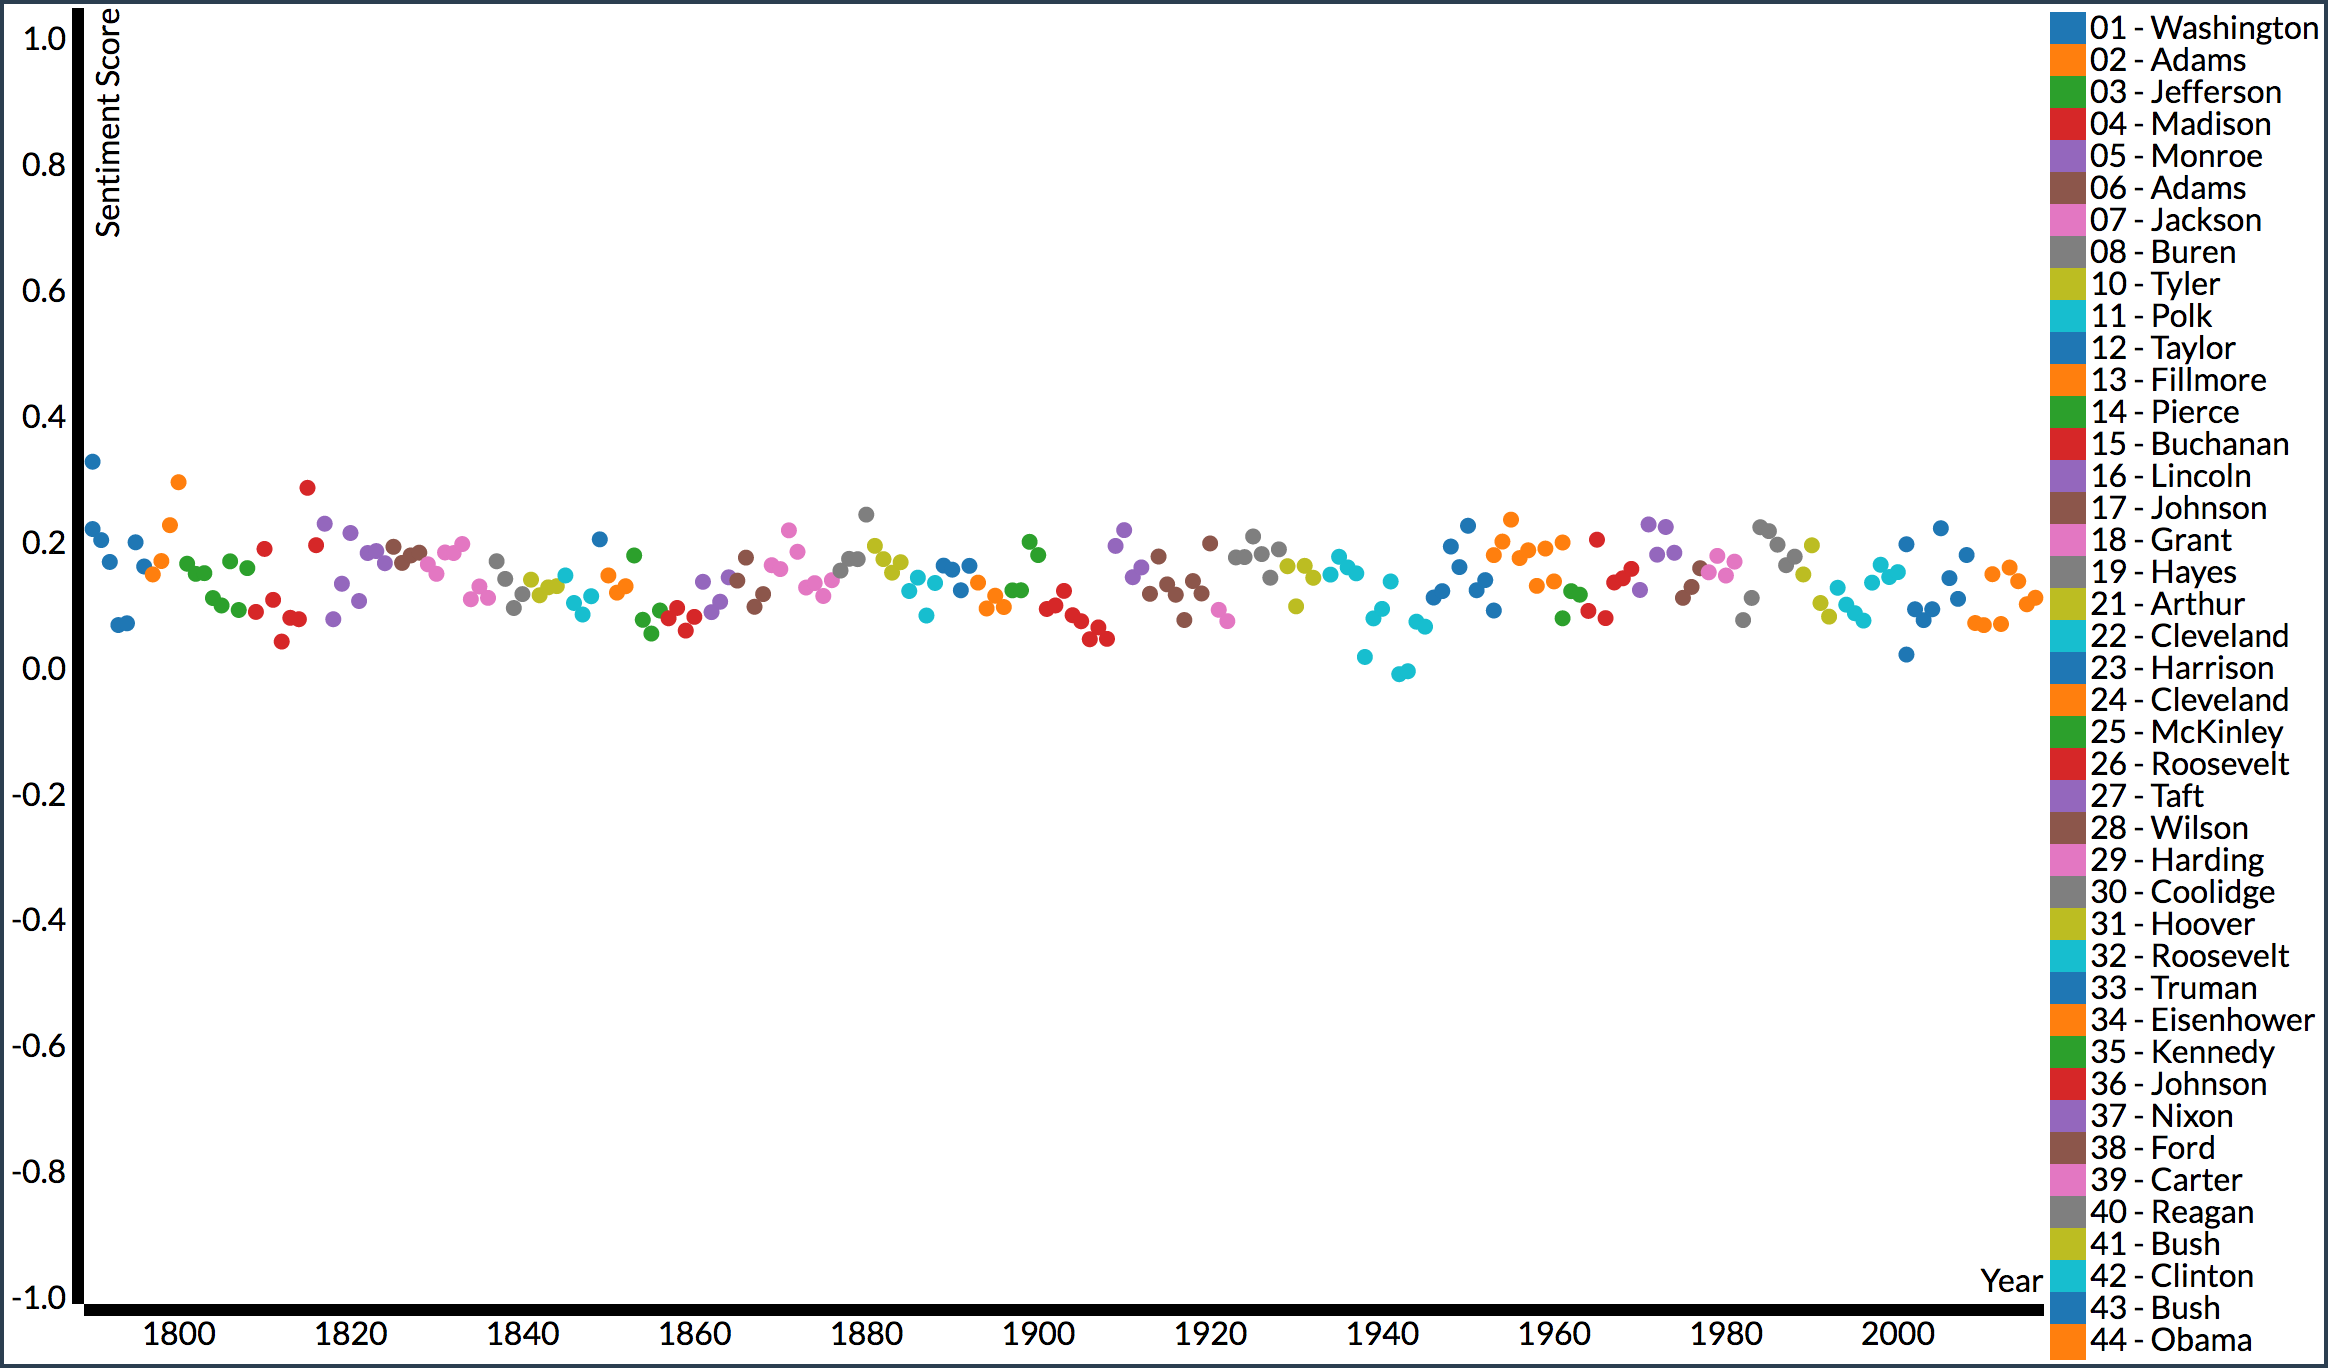
\includegraphics[width=\columnwidth]{images/Lineplot.png}
  \caption{Line Plot}
  \label{fig:lineplot1}
\end{figure}
Line plots are effective at showing data over time and it allows for users to see overall trends in tone and compare the scores across presidencies to see tonal shifts over a president's tenure or how two presidents compared to one another.
The data set lends itself to this representation and the result is a nice longitudinal summary of presidential tones over the course of history.
The data being displayed isn't objective and it must be taken with a grain of salt because sentiment analysis is far from an exact science and the lexicon is objective but also doesn't take in to account the change of meaning seen in some words.
The time period for these changes is a relatively short period of time in the context of language so the differences shouldn't be greatly significant in the shifting of tone but it is something to note.
The Line plot itself also allows for interaction in that the user can hover over a point and get detailed information about it, such as the President's name, the term and year that address was delivered, as well as the exact sentiment score.
Beyond this line plot representation, this speech data was also used to create another visual that isn't as objectively meaningful and helpful, but does provide some context with word usage and a fun visual to see, and that is word clouds.

\subsection{Word Cloud}
A word cloud is a collage of words that displays word frequencies for a certain set of text data, with the relative size of each word being determined by the frequency with which that term is used in the text.
An example can be seen in figure FIGURE that shows the word cloud for PRESIDENT AND TERM.
Word Clouds are an interesting visual since they provide quick reference to see what a President's most used terms are, as well as being another interesting way to engage the data in a slightly different context.
Word Clouds themselves are often criticized since it is a poor way to visualize data and it is hard to objectively compare two words in a word cloud because the frequency values are encoded using area, which is a very difficult encoding for humans to interpret.
In this case, the word cloud is used merely to complement the existing line plot visualization that provides insight into the main purpose of the research, and the word cloud provides a different way of visualizing the data source itself.

\subsection{D3}
D3.js (D3) is the JavaScript Library used to create the two visualizations mentioned in the previous sections.
D3 uses pre-built JavaScript functions to select, elements, create SVG elements, style them, or add dynamic effects or tooltips to them [\cite{bostock2011d3}].
This tooltip functionality was used in the line plot demonstration mentioned previously to give extra information on each data point without cluttering the visualization itself.
Another feature implemented using D3 is that if the user hovers over a President's name, then just that President's data points will be highlighted and the rest are faded out of the screen.
D3 also has a handy library that creates word clouds that was used in this research, it takes in an input array in JSON format with the words and their frequencies in decreasing order and draws the words with their relative sizes on the HTML canvas.
There is a bit of a delay on the drawing of the word clouds, since instead of saved images of the word clouds, the program is actually drawing all of them in realtime and just swapping out the JSON data source depending on which President is selected in the dropdown menu at the top of the page.

\section{State of the Union Addresses}
The main textual data that was collected to be processed was all of the Presidential State of the Unions from George Washington's first address to Barack Obama's last address.
The text source was initially pulled from a \href{http://stateoftheunion.onetwothree.net/appendices.html#source}{Presidential Address Repository}.
The text came in a large text file that contained every speech and it was split in to individual text files for each individual address to allow for easier processing.
The addresses vary widely in length and content, which is also of significant note when analyzing and comparing these addresses across the timespan of the existence of the United States.
George Washington's first address was just over a thousand words and seventeen paragraphs, whereas Barack Obama's final address was just over 5,400 words and was 78 paragraphs long.

\subsection{Change in Purpose of State of the Union Address}
The length is the most notable change in the State of the Union Addresses over time, but there are important factors to consider as well that could potentially impact how the addresses are given from year to year.
When the Presidential Addresses first started with George Washington, it was not supposed to be a recurring event [\cite{teten2003evolution}], but it soon began to grow to a tradition so that the president could publicly address the people and inform them of the current events of the country.
Over the years, the Presidential Address has taken on many forms, in spoken word, in written letter, in radio broadcast, and, nowadays, on live television broadcast.
The Presidential Address shifted from the yearly Presidential update, sometimes the only times people would hear directly from the President, to a formalized briefing to inform the public in an organized manner of the current state of affairs and push forward a President's agenda for the upcoming term [\cite{teten2003evolution}].
While that has always been somewhat of the purpose of the addresses, it has become more of the central focus over the course of time due to technological innovations and changes in media coverage.
Nowadays, citizens of the United States can read in real-time about the decisions of the Presidency and the Presidents political moves without needing to listen to a one time speech to become updated on their agenda and goals for the year to come.
It is a subtle, yet interesting shift in how the addresses are approached and given, but even these purposes could change between years depending on the person giving these orations, an important factor to consider also.

\subsection{Presidential Personality}
Another important factor in how the Presidential State of the Union Addresses are given is the personality of the President that is giving them.
This is a rather intangible element of the speeches that can be hard to quantify but is very important to note.
Most people have a certain disposition towards being on the more optimistic or pessimistic side of life and that can display itself in the speeches given.
Since the important topic being considered here is tone, that can be heavily influenced by if the President giving the speech tends to be more realistic or optimistic in their outlook on the world, and to potentially create a better one.
Some President's may see the State of the Union as a chance to rally the nation and drum positivity and support for their platform for years to come, whereas others might see it as a good opportunity to have a nation-wide reality check and bring the citizens in-line with what needs to be done for the good of the nation [\cite{teten2003evolution}].

\subsection{Summary of Data}
It is important to have an understanding of the speech data itself before diving in to this research, since otherwise it won't be as meaningful and will be harder to draw conclusions from it. Here (Reference to Stat Chart) is a chart containing a statistical summary for the important features of the data set that are relevant to this research.
This can be explored to search for trends in the data and familiarize oneself with an overall perspective on the data.
Some information of note: 
There are a total of 230 Presidential Addresses given by 42 Presidents, making the average number of addresses per president 5. 
There are 26 Republicans and 16 Democrats , which makes their percentages 62\% and 38\%, respectively.
The average length of speech is AVGLENG and the average sentiment score of every address is OVERALLAVG.
An extended statistical overview can be found here (Link to Statistics Section)

\section{Machine Learning}

\subsection{Naives Bayes}

\subsection{Neural Network}

\subsection{Decision Tree}

\begin{comment}
The process in its simplest form isn't very complex, but it is important to establish the principles that guide a sentiment analysis.
In the most basic of terms, a sample of text is taken and tokenized and evaluated

\section{State of the Union Addresses}
% sentiment analysis lexicons and stuff - definitions of issue of working with text data and big text data
% kinds of things you do 
% what all do I need to include
% Background - what are state of the unions and why are they important
% give some data were democrat and how many were republican
% how chose to account for the different parties
% What information do I need to know about before I understand what I'm about to be presented
% Natural language processing
% political leaning
% sentiment analysis
% wHat everybody else did and what needs to be understood to go from here
% references where you talk about information visualization
% most of the effort in the writing of the paper
% most of bibliography entries
The main textual data that was collected to be processed was all of the Presidential State of the Unions from George Washington's first address to Barack Obama's last address.
The text source was initially pulled from a \href{http://stateoftheunion.onetwothree.net/appendices.html#source}{Presidential Address Repository}.


\section{Topic Classifier Sets}
An important part of the latter half of the preprocessing work for this research was the topic classifier sets.
At first, the sentiment score was calculated for each presidential address with an overall score from -1 to 1, indicating their tone when delivering that address.
After these were calculated, they were analyzed to look for trends in each president's tone to see if there were any interesting observations to be seen.
As an additional breakdown to see if there was any more context-specific information that could help determine a president's political party, topic categories were added to diversify the scores of the president's even more.

Four Presidential Addresses were chosen (Washington, Lincoln, Kennedy, Obama) and manually read through to discover what words were being used when talking about certain topics within the United States. The topics that were chosen were: crime, economy, education, energy, environment, family, foreign, government, job, religion, terrorism, and war. Text files were created using the trigger words for each major topic, the trigger words being pulled from the four addresses mentioned above and throughout various other addresses as they were skimmed through, that would add the entire sentence to an array named for what topic it was going to collect information on. This processing was conducted on every address and the sentiment score for each topic was found for each president, which resulted in a vector for each address that had their overall sentiment score and the sentiment score for each topic covered in the address. These scores for each address were then averaged together to create an overall vector for each president that could be used for classification and learning to learn their political party and predict others.
\end{comment}